\documentclass[1p]{elsarticle_modified}
%\bibliographystyle{elsarticle-num}

%\usepackage[colorlinks]{hyperref}
%\usepackage{abbrmath_seonhwa} %\Abb, \Ascr, \Acal ,\Abf, \Afrak
\usepackage{amsfonts}
\usepackage{amssymb}
\usepackage{amsmath}
\usepackage{amsthm}
\usepackage{scalefnt}
\usepackage{amsbsy}
\usepackage{kotex}
\usepackage{caption}
\usepackage{subfig}
\usepackage{color}
\usepackage{graphicx}
\usepackage{xcolor} %% white, black, red, green, blue, cyan, magenta, yellow
\usepackage{float}
\usepackage{setspace}
\usepackage{hyperref}

\usepackage{tikz}
\usetikzlibrary{arrows}

\usepackage{multirow}
\usepackage{array} % fixed length table
\usepackage{hhline}

%%%%%%%%%%%%%%%%%%%%%
\makeatletter
\renewcommand*\env@matrix[1][\arraystretch]{%
	\edef\arraystretch{#1}%
	\hskip -\arraycolsep
	\let\@ifnextchar\new@ifnextchar
	\array{*\c@MaxMatrixCols c}}
\makeatother %https://tex.stackexchange.com/questions/14071/how-can-i-increase-the-line-spacing-in-a-matrix
%%%%%%%%%%%%%%%

\usepackage[normalem]{ulem}

\newcommand{\msout}[1]{\ifmmode\text{\sout{\ensuremath{#1}}}\else\sout{#1}\fi}
%SOURCE: \msout is \stkout macro in https://tex.stackexchange.com/questions/20609/strikeout-in-math-mode

\newcommand{\cancel}[1]{
	\ifmmode
	{\color{red}\msout{#1}}
	\else
	{\color{red}\sout{#1}}
	\fi
}

\newcommand{\add}[1]{
	{\color{blue}\uwave{#1}}
}

\newcommand{\replace}[2]{
	\ifmmode
	{\color{red}\msout{#1}}{\color{blue}\uwave{#2}}
	\else
	{\color{red}\sout{#1}}{\color{blue}\uwave{#2}}
	\fi
}

\newcommand{\Sol}{\mathcal{S}} %segment
\newcommand{\D}{D} %diagram
\newcommand{\A}{\mathcal{A}} %arc


%%%%%%%%%%%%%%%%%%%%%%%%%%%%%5 test

\def\sl{\operatorname{\textup{SL}}(2,\Cbb)}
\def\psl{\operatorname{\textup{PSL}}(2,\Cbb)}
\def\quan{\mkern 1mu \triangleright \mkern 1mu}

\theoremstyle{definition}
\newtheorem{thm}{Theorem}[section]
\newtheorem{prop}[thm]{Proposition}
\newtheorem{lem}[thm]{Lemma}
\newtheorem{ques}[thm]{Question}
\newtheorem{cor}[thm]{Corollary}
\newtheorem{defn}[thm]{Definition}
\newtheorem{exam}[thm]{Example}
\newtheorem{rmk}[thm]{Remark}
\newtheorem{alg}[thm]{Algorithm}

\newcommand{\I}{\sqrt{-1}}
\begin{document}

%\begin{frontmatter}
%
%\title{Boundary parabolic representations of knots up to 8 crossings}
%
%%% Group authors per affiliation:
%\author{Yunhi Cho} 
%\address{Department of Mathematics, University of Seoul, Seoul, Korea}
%\ead{yhcho@uos.ac.kr}
%
%
%\author{Seonhwa Kim} %\fnref{s_kim}}
%\address{Center for Geometry and Physics, Institute for Basic Science, Pohang, 37673, Korea}
%\ead{ryeona17@ibs.re.kr}
%
%\author{Hyuk Kim}
%\address{Department of Mathematical Sciences, Seoul National University, Seoul 08826, Korea}
%\ead{hyukkim@snu.ac.kr}
%
%\author{Seokbeom Yoon}
%\address{Department of Mathematical Sciences, Seoul National University, Seoul, 08826,  Korea}
%\ead{sbyoon15@snu.ac.kr}
%
%\begin{abstract}
%We find all boundary parabolic representation of knots up to 8 crossings.
%
%\end{abstract}
%\begin{keyword}
%    \MSC[2010] 57M25 
%\end{keyword}
%
%\end{frontmatter}

%\linenumbers
%\tableofcontents
%
\newcommand\colored[1]{\textcolor{white}{\rule[-0.35ex]{0.8em}{1.4ex}}\kern-0.8em\color{red} #1}%
%\newcommand\colored[1]{\textcolor{white}{ #1}\kern-2.17ex	\textcolor{white}{ #1}\kern-1.81ex	\textcolor{white}{ #1}\kern-2.15ex\color{red}#1	}

{\Large $\underline{11a_{301}~(K11a_{301})}$}

\setlength{\tabcolsep}{10pt}
\renewcommand{\arraystretch}{1.6}
\vspace{1cm}\begin{tabular}{m{100pt}>{\centering\arraybackslash}m{274pt}}
\multirow{5}{120pt}{
	\centering
	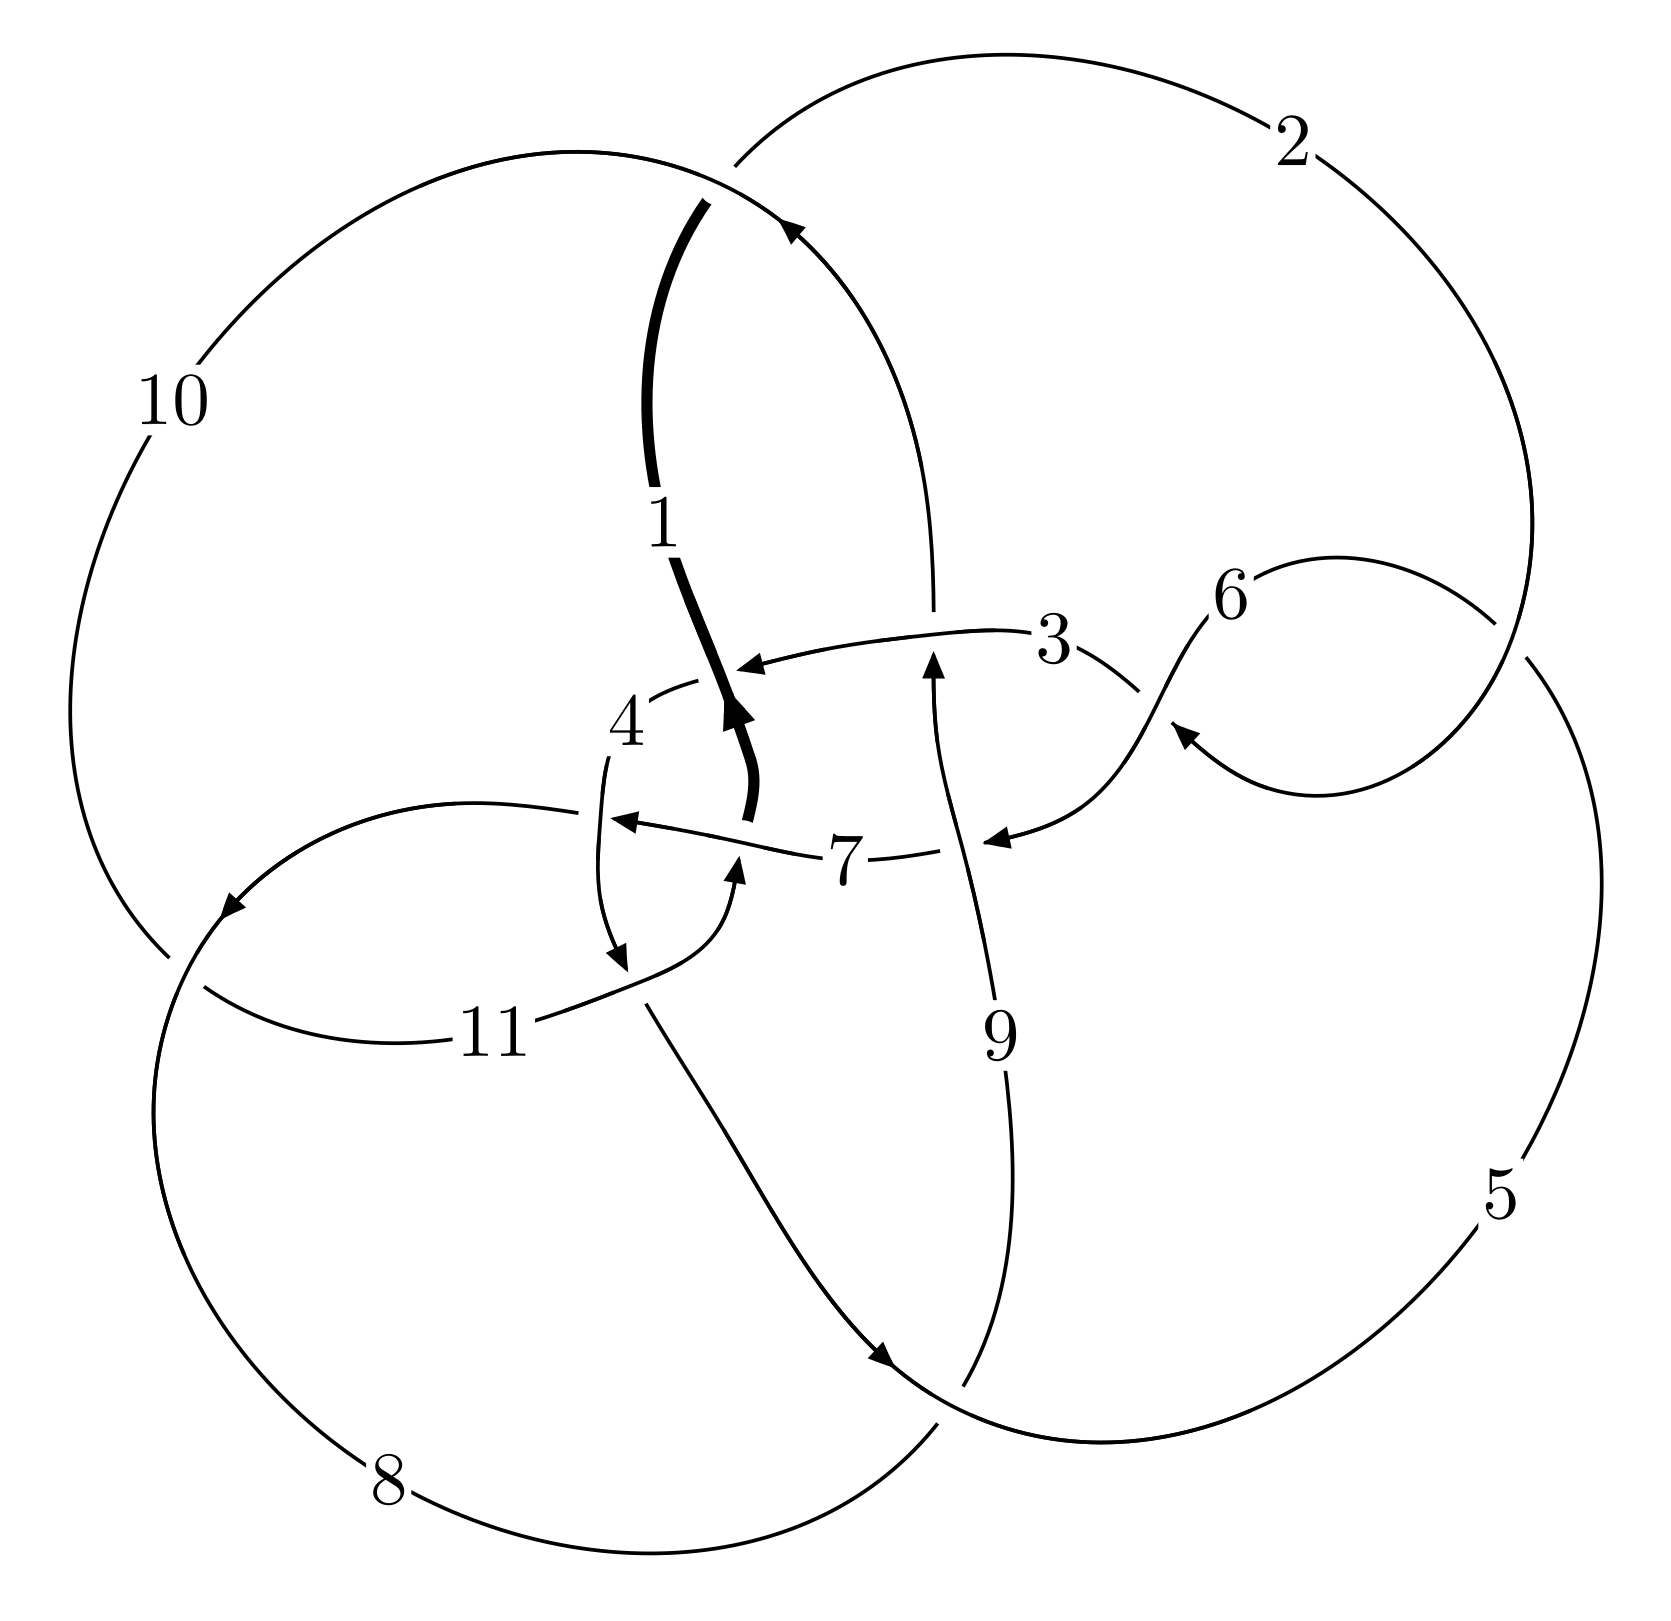
\includegraphics[width=112pt]{../../../GIT/diagram.site/Diagrams/png/550_11a_301.png}\\
\ \ \ A knot diagram\footnotemark}&
\allowdisplaybreaks
\textbf{Linearized knot diagam} \\
\cline{2-2}
 &
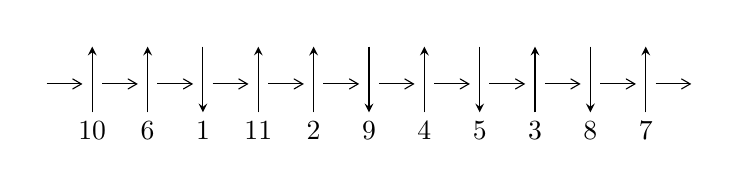
\begin{tikzpicture}[x=20pt, y=17pt]
	% nodes
	\node (C0) at (0, 0) {};
	\node (C1) at (1, 0) {};
	\node (C1U) at (1, +1) {};
	\node (C1D) at (1, -1) {10};

	\node (C2) at (2, 0) {};
	\node (C2U) at (2, +1) {};
	\node (C2D) at (2, -1) {6};

	\node (C3) at (3, 0) {};
	\node (C3U) at (3, +1) {};
	\node (C3D) at (3, -1) {1};

	\node (C4) at (4, 0) {};
	\node (C4U) at (4, +1) {};
	\node (C4D) at (4, -1) {11};

	\node (C5) at (5, 0) {};
	\node (C5U) at (5, +1) {};
	\node (C5D) at (5, -1) {2};

	\node (C6) at (6, 0) {};
	\node (C6U) at (6, +1) {};
	\node (C6D) at (6, -1) {9};

	\node (C7) at (7, 0) {};
	\node (C7U) at (7, +1) {};
	\node (C7D) at (7, -1) {4};

	\node (C8) at (8, 0) {};
	\node (C8U) at (8, +1) {};
	\node (C8D) at (8, -1) {5};

	\node (C9) at (9, 0) {};
	\node (C9U) at (9, +1) {};
	\node (C9D) at (9, -1) {3};

	\node (C10) at (10, 0) {};
	\node (C10U) at (10, +1) {};
	\node (C10D) at (10, -1) {8};

	\node (C11) at (11, 0) {};
	\node (C11U) at (11, +1) {};
	\node (C11D) at (11, -1) {7};
	\node (C12) at (12, 0) {};

	% arrows
	\draw[->,>={angle 60}]
	(C0) edge (C1) (C1) edge (C2) (C2) edge (C3) (C3) edge (C4) (C4) edge (C5) (C5) edge (C6) (C6) edge (C7) (C7) edge (C8) (C8) edge (C9) (C9) edge (C10) (C10) edge (C11) (C11) edge (C12) ;	\draw[->,>=stealth]
	(C1D) edge (C1U) (C2D) edge (C2U) (C3U) edge (C3D) (C4D) edge (C4U) (C5D) edge (C5U) (C6U) edge (C6D) (C7D) edge (C7U) (C8U) edge (C8D) (C9D) edge (C9U) (C10U) edge (C10D) (C11D) edge (C11U) ;
	\end{tikzpicture} \\
\hhline{~~} \\& 
\textbf{Solving Sequence} \\ \cline{2-2} 
 &
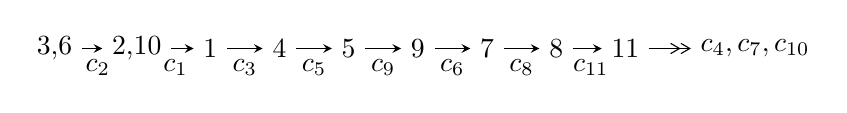
\begin{tikzpicture}[x=25pt, y=7pt]
	% node
	\node (A0) at (-1/8, 0) {3,6};
	\node (A1) at (17/16, 0) {2,10};
	\node (A2) at (17/8, 0) {1};
	\node (A3) at (25/8, 0) {4};
	\node (A4) at (33/8, 0) {5};
	\node (A5) at (41/8, 0) {9};
	\node (A6) at (49/8, 0) {7};
	\node (A7) at (57/8, 0) {8};
	\node (A8) at (65/8, 0) {11};
	\node (C1) at (1/2, -1) {$c_{2}$};
	\node (C2) at (13/8, -1) {$c_{1}$};
	\node (C3) at (21/8, -1) {$c_{3}$};
	\node (C4) at (29/8, -1) {$c_{5}$};
	\node (C5) at (37/8, -1) {$c_{9}$};
	\node (C6) at (45/8, -1) {$c_{6}$};
	\node (C7) at (53/8, -1) {$c_{8}$};
	\node (C8) at (61/8, -1) {$c_{11}$};
	\node (A9) at (10, 0) {$c_{4},c_{7},c_{10}$};

	% edge
	\draw[->,>=stealth]	
	(A0) edge (A1) (A1) edge (A2) (A2) edge (A3) (A3) edge (A4) (A4) edge (A5) (A5) edge (A6) (A6) edge (A7) (A7) edge (A8) ;
	\draw[->>,>={angle 60}]	
	(A8) edge (A9);
\end{tikzpicture} \\ 

\end{tabular} \\

\footnotetext{
The image of knot diagram is generated by the software ``\textbf{Draw programme}" developed by Andrew Bartholomew(\url{http://www.layer8.co.uk/maths/draw/index.htm\#Running-draw}), where we modified some parts for our purpose(\url{https://github.com/CATsTAILs/LinksPainter}).
}\phantom \\ \newline 
\centering \textbf{Ideals for irreducible components\footnotemark of $X_{\text{par}}$} 
 
\begin{align*}
I^u_{1}&=\langle 
-1.16899\times10^{426} u^{123}+3.22194\times10^{424} u^{122}+\cdots+2.77126\times10^{424} b-1.62179\times10^{428},\\
\phantom{I^u_{1}}&\phantom{= \langle  }-3.58082\times10^{428} u^{123}+4.35420\times10^{427} u^{122}+\cdots+3.85206\times10^{426} a-5.63094\times10^{430},\\
\phantom{I^u_{1}}&\phantom{= \langle  }u^{124}- u^{123}+\cdots+72 u-139\rangle \\
I^u_{2}&=\langle 
-9566660926250 u^{24}-22937945374331 u^{23}+\cdots+19862837987731 b-37700474512606,\\
\phantom{I^u_{2}}&\phantom{= \langle  }18263853921862 u^{24}-37210165575977 u^{23}+\cdots+19862837987731 a-129534774263607,\\
\phantom{I^u_{2}}&\phantom{= \langle  }u^{25}-7 u^{23}+\cdots-2 u-1\rangle \\
\\
\end{align*}
\raggedright * 2 irreducible components of $\dim_{\mathbb{C}}=0$, with total 149 representations.\\
\footnotetext{All coefficients of polynomials are rational numbers. But the coefficients are sometimes approximated in decimal forms when there is not enough margin.}
\newpage
\renewcommand{\arraystretch}{1}
\centering \section*{I. $I^u_{1}= \langle -1.17\times10^{426} u^{123}+3.22\times10^{424} u^{122}+\cdots+2.77\times10^{424} b-1.62\times10^{428},\;-3.58\times10^{428} u^{123}+4.35\times10^{427} u^{122}+\cdots+3.85\times10^{426} a-5.63\times10^{430},\;u^{124}- u^{123}+\cdots+72 u-139 \rangle$}
\flushleft \textbf{(i) Arc colorings}\\
\begin{tabular}{m{7pt} m{180pt} m{7pt} m{180pt} }
\flushright $a_{3}=$&$\begin{pmatrix}1\\0\end{pmatrix}$ \\
\flushright $a_{6}=$&$\begin{pmatrix}0\\u\end{pmatrix}$ \\
\flushright $a_{2}=$&$\begin{pmatrix}1\\u^2\end{pmatrix}$ \\
\flushright $a_{10}=$&$\begin{pmatrix}92.9586 u^{123}-11.3036 u^{122}+\cdots+8759.18 u+14618.0\\42.1826 u^{123}-1.16263 u^{122}+\cdots+2521.74 u+5852.16\end{pmatrix}$ \\
\flushright $a_{1}=$&$\begin{pmatrix}-5.00646 u^{123}+4.79793 u^{122}+\cdots-2365.30 u-1732.01\\-31.9252 u^{123}+10.1950 u^{122}+\cdots-5531.06 u-6308.34\end{pmatrix}$ \\
\flushright $a_{4}=$&$\begin{pmatrix}-124.235 u^{123}+22.8343 u^{122}+\cdots-15054.5 u-21208.6\\-85.2237 u^{123}+10.8039 u^{122}+\cdots-8254.49 u-13491.4\end{pmatrix}$ \\
\flushright $a_{5}=$&$\begin{pmatrix}- u\\- u^3+u\end{pmatrix}$ \\
\flushright $a_{9}=$&$\begin{pmatrix}50.7760 u^{123}-10.1409 u^{122}+\cdots+6237.44 u+8765.86\\42.1826 u^{123}-1.16263 u^{122}+\cdots+2521.74 u+5852.16\end{pmatrix}$ \\
\flushright $a_{7}=$&$\begin{pmatrix}34.5243 u^{123}-6.25865 u^{122}+\cdots+3698.51 u+5768.67\\11.4223 u^{123}-0.700100 u^{122}+\cdots+943.261 u+1677.60\end{pmatrix}$ \\
\flushright $a_{8}=$&$\begin{pmatrix}102.195 u^{123}-14.9472 u^{122}+\cdots+10619.6 u+16588.2\\32.7163 u^{123}-0.757045 u^{122}+\cdots+1930.76 u+4508.98\end{pmatrix}$ \\
\flushright $a_{11}=$&$\begin{pmatrix}-19.4270 u^{123}+10.0533 u^{122}+\cdots-5043.28 u-4731.63\\-16.2148 u^{123}+7.73509 u^{122}+\cdots-3918.69 u-3758.08\end{pmatrix}$\\ \flushright $a_{11}=$&$\begin{pmatrix}-19.4270 u^{123}+10.0533 u^{122}+\cdots-5043.28 u-4731.63\\-16.2148 u^{123}+7.73509 u^{122}+\cdots-3918.69 u-3758.08\end{pmatrix}$\\&\end{tabular}
\flushleft \textbf{(ii) Obstruction class $= -1$}\\~\\
\flushleft \textbf{(iii) Cusp Shapes $= -3231.64 u^{123}+356.760 u^{122}+\cdots-305355. u-504514.$}\\~\\
\newpage\renewcommand{\arraystretch}{1}
\flushleft \textbf{(iv) u-Polynomials at the component}\newline \\
\begin{tabular}{m{50pt}|m{274pt}}
Crossings & \hspace{64pt}u-Polynomials at each crossing \\
\hline $$\begin{aligned}c_{1}\end{aligned}$$&$\begin{aligned}
&u^{124}-4 u^{123}+\cdots-479 u+107
\end{aligned}$\\
\hline $$\begin{aligned}c_{2},c_{5}\end{aligned}$$&$\begin{aligned}
&u^{124}- u^{123}+\cdots+72 u-139
\end{aligned}$\\
\hline $$\begin{aligned}c_{3}\end{aligned}$$&$\begin{aligned}
&u^{124}-9 u^{123}+\cdots+97 u-1
\end{aligned}$\\
\hline $$\begin{aligned}c_{4}\end{aligned}$$&$\begin{aligned}
&u^{124}- u^{123}+\cdots+154 u+19
\end{aligned}$\\
\hline $$\begin{aligned}c_{6}\end{aligned}$$&$\begin{aligned}
&u^{124}+3 u^{123}+\cdots-5094 u+1919
\end{aligned}$\\
\hline $$\begin{aligned}c_{7}\end{aligned}$$&$\begin{aligned}
&u^{124}-3 u^{123}+\cdots+19 u-1
\end{aligned}$\\
\hline $$\begin{aligned}c_{8}\end{aligned}$$&$\begin{aligned}
&u^{124}- u^{123}+\cdots+104 u+13
\end{aligned}$\\
\hline $$\begin{aligned}c_{9}\end{aligned}$$&$\begin{aligned}
&u^{124}-13 u^{122}+\cdots-27900 u-5737
\end{aligned}$\\
\hline $$\begin{aligned}c_{10}\end{aligned}$$&$\begin{aligned}
&u^{124}+3 u^{123}+\cdots-26 u-5
\end{aligned}$\\
\hline $$\begin{aligned}c_{11}\end{aligned}$$&$\begin{aligned}
&u^{124}+u^{123}+\cdots-23 u-1
\end{aligned}$\\
\hline
\end{tabular}\\~\\
\newpage\renewcommand{\arraystretch}{1}
\flushleft \textbf{(v) Riley Polynomials at the component}\newline \\
\begin{tabular}{m{50pt}|m{274pt}}
Crossings & \hspace{64pt}Riley Polynomials at each crossing \\
\hline $$\begin{aligned}c_{1}\end{aligned}$$&$\begin{aligned}
&y^{124}-32 y^{123}+\cdots-782845 y+11449
\end{aligned}$\\
\hline $$\begin{aligned}c_{2},c_{5}\end{aligned}$$&$\begin{aligned}
&y^{124}-75 y^{123}+\cdots-605108 y+19321
\end{aligned}$\\
\hline $$\begin{aligned}c_{3}\end{aligned}$$&$\begin{aligned}
&y^{124}+27 y^{123}+\cdots-8505 y+1
\end{aligned}$\\
\hline $$\begin{aligned}c_{4}\end{aligned}$$&$\begin{aligned}
&y^{124}+3 y^{123}+\cdots+15842 y+361
\end{aligned}$\\
\hline $$\begin{aligned}c_{6}\end{aligned}$$&$\begin{aligned}
&y^{124}+11 y^{123}+\cdots+56088414 y+3682561
\end{aligned}$\\
\hline $$\begin{aligned}c_{7}\end{aligned}$$&$\begin{aligned}
&y^{124}-17 y^{123}+\cdots-287 y+1
\end{aligned}$\\
\hline $$\begin{aligned}c_{8}\end{aligned}$$&$\begin{aligned}
&y^{124}-23 y^{123}+\cdots+29224 y+169
\end{aligned}$\\
\hline $$\begin{aligned}c_{9}\end{aligned}$$&$\begin{aligned}
&y^{124}-26 y^{123}+\cdots+93166514 y+32913169
\end{aligned}$\\
\hline $$\begin{aligned}c_{10}\end{aligned}$$&$\begin{aligned}
&y^{124}-5 y^{123}+\cdots-7526 y+25
\end{aligned}$\\
\hline $$\begin{aligned}c_{11}\end{aligned}$$&$\begin{aligned}
&y^{124}-7 y^{123}+\cdots-113 y+1
\end{aligned}$\\
\hline
\end{tabular}\\~\\
\newpage\flushleft \textbf{(vi) Complex Volumes and Cusp Shapes}
$$\begin{array}{c|c|c}  
\text{Solutions to }I^u_{1}& \I (\text{vol} + \sqrt{-1}CS) & \text{Cusp shape}\\
 \hline 
\begin{aligned}
u &= \phantom{-}0.974071 + 0.190755 I \\
a &= -0.550421 - 0.599368 I \\
b &= \phantom{-}0.18852 - 1.65134 I\end{aligned}
 & -0.577215 + 1.239640 I & \phantom{-0.000000 } 0 \\ \hline\begin{aligned}
u &= \phantom{-}0.974071 - 0.190755 I \\
a &= -0.550421 + 0.599368 I \\
b &= \phantom{-}0.18852 + 1.65134 I\end{aligned}
 & -0.577215 - 1.239640 I & \phantom{-0.000000 } 0 \\ \hline\begin{aligned}
u &= -0.902521 + 0.400409 I \\
a &= -0.609673 - 1.244710 I \\
b &= -1.054330 + 0.045528 I\end{aligned}
 & \phantom{-}3.54338 + 2.85043 I & \phantom{-0.000000 } 0 \\ \hline\begin{aligned}
u &= -0.902521 - 0.400409 I \\
a &= -0.609673 + 1.244710 I \\
b &= -1.054330 - 0.045528 I\end{aligned}
 & \phantom{-}3.54338 - 2.85043 I & \phantom{-0.000000 } 0 \\ \hline\begin{aligned}
u &= \phantom{-}0.415249 + 0.881418 I \\
a &= \phantom{-}0.306635 + 0.205268 I \\
b &= -0.737227 - 0.595686 I\end{aligned}
 & \phantom{-}1.58492 + 6.17096 I & \phantom{-0.000000 } 0 \\ \hline\begin{aligned}
u &= \phantom{-}0.415249 - 0.881418 I \\
a &= \phantom{-}0.306635 - 0.205268 I \\
b &= -0.737227 + 0.595686 I\end{aligned}
 & \phantom{-}1.58492 - 6.17096 I & \phantom{-0.000000 } 0 \\ \hline\begin{aligned}
u &= -1.026590 + 0.019415 I \\
a &= \phantom{-}1.30114 - 1.03924 I \\
b &= \phantom{-}0.811133 + 0.640015 I\end{aligned}
 & \phantom{-}4.16687 + 3.71959 I & \phantom{-0.000000 } 0 \\ \hline\begin{aligned}
u &= -1.026590 - 0.019415 I \\
a &= \phantom{-}1.30114 + 1.03924 I \\
b &= \phantom{-}0.811133 - 0.640015 I\end{aligned}
 & \phantom{-}4.16687 - 3.71959 I & \phantom{-0.000000 } 0 \\ \hline\begin{aligned}
u &= -0.967014 + 0.360220 I \\
a &= -1.129450 + 0.668006 I \\
b &= -0.017238 - 0.228701 I\end{aligned}
 & -0.31910 - 5.18786 I & \phantom{-0.000000 } 0 \\ \hline\begin{aligned}
u &= -0.967014 - 0.360220 I \\
a &= -1.129450 - 0.668006 I \\
b &= -0.017238 + 0.228701 I\end{aligned}
 & -0.31910 + 5.18786 I & \phantom{-0.000000 } 0\\
 \hline 
 \end{array}$$\newpage$$\begin{array}{c|c|c}  
\text{Solutions to }I^u_{1}& \I (\text{vol} + \sqrt{-1}CS) & \text{Cusp shape}\\
 \hline 
\begin{aligned}
u &= \phantom{-}1.018330 + 0.170276 I \\
a &= -2.51955 - 0.33224 I \\
b &= -1.51339 - 0.05960 I\end{aligned}
 & \phantom{-}1.91161 + 3.30620 I & \phantom{-0.000000 } 0 \\ \hline\begin{aligned}
u &= \phantom{-}1.018330 - 0.170276 I \\
a &= -2.51955 + 0.33224 I \\
b &= -1.51339 + 0.05960 I\end{aligned}
 & \phantom{-}1.91161 - 3.30620 I & \phantom{-0.000000 } 0 \\ \hline\begin{aligned}
u &= -0.981740 + 0.336373 I \\
a &= \phantom{-}0.141564 + 0.271103 I \\
b &= \phantom{-}0.172395 - 0.978948 I\end{aligned}
 & \phantom{-}0.03669 - 4.64999 I & \phantom{-0.000000 } 0 \\ \hline\begin{aligned}
u &= -0.981740 - 0.336373 I \\
a &= \phantom{-}0.141564 - 0.271103 I \\
b &= \phantom{-}0.172395 + 0.978948 I\end{aligned}
 & \phantom{-}0.03669 + 4.64999 I & \phantom{-0.000000 } 0 \\ \hline\begin{aligned}
u &= -1.003740 + 0.303527 I \\
a &= \phantom{-}0.137773 + 1.402230 I \\
b &= \phantom{-}0.58661 + 1.97658 I\end{aligned}
 & \phantom{-}0.79053 - 10.52770 I & \phantom{-0.000000 } 0 \\ \hline\begin{aligned}
u &= -1.003740 - 0.303527 I \\
a &= \phantom{-}0.137773 - 1.402230 I \\
b &= \phantom{-}0.58661 - 1.97658 I\end{aligned}
 & \phantom{-}0.79053 + 10.52770 I & \phantom{-0.000000 } 0 \\ \hline\begin{aligned}
u &= \phantom{-}0.279917 + 0.908578 I \\
a &= -0.083523 + 0.475369 I \\
b &= \phantom{-}0.643948 + 0.220659 I\end{aligned}
 & \phantom{-}0.412874 + 0.819655 I & \phantom{-0.000000 } 0 \\ \hline\begin{aligned}
u &= \phantom{-}0.279917 - 0.908578 I \\
a &= -0.083523 - 0.475369 I \\
b &= \phantom{-}0.643948 - 0.220659 I\end{aligned}
 & \phantom{-}0.412874 - 0.819655 I & \phantom{-0.000000 } 0 \\ \hline\begin{aligned}
u &= \phantom{-}0.922490 + 0.200559 I \\
a &= \phantom{-}3.33471 + 0.42892 I \\
b &= \phantom{-}0.366441 + 0.434684 I\end{aligned}
 & \phantom{-}0.58612 + 9.17333 I & \phantom{-0.000000 } 0 \\ \hline\begin{aligned}
u &= \phantom{-}0.922490 - 0.200559 I \\
a &= \phantom{-}3.33471 - 0.42892 I \\
b &= \phantom{-}0.366441 - 0.434684 I\end{aligned}
 & \phantom{-}0.58612 - 9.17333 I & \phantom{-0.000000 } 0\\
 \hline 
 \end{array}$$\newpage$$\begin{array}{c|c|c}  
\text{Solutions to }I^u_{1}& \I (\text{vol} + \sqrt{-1}CS) & \text{Cusp shape}\\
 \hline 
\begin{aligned}
u &= \phantom{-}0.378914 + 0.858907 I \\
a &= -0.115862 - 0.434906 I \\
b &= \phantom{-}1.108480 - 0.790196 I\end{aligned}
 & -0.68132 - 4.84270 I & \phantom{-0.000000 } 0 \\ \hline\begin{aligned}
u &= \phantom{-}0.378914 - 0.858907 I \\
a &= -0.115862 + 0.434906 I \\
b &= \phantom{-}1.108480 + 0.790196 I\end{aligned}
 & -0.68132 + 4.84270 I & \phantom{-0.000000 } 0 \\ \hline\begin{aligned}
u &= -0.130351 + 1.065560 I \\
a &= \phantom{-}0.1316640 - 0.0246824 I \\
b &= -0.928596 - 0.693787 I\end{aligned}
 & -1.66000 + 5.39588 I & \phantom{-0.000000 } 0 \\ \hline\begin{aligned}
u &= -0.130351 - 1.065560 I \\
a &= \phantom{-}0.1316640 + 0.0246824 I \\
b &= -0.928596 + 0.693787 I\end{aligned}
 & -1.66000 - 5.39588 I & \phantom{-0.000000 } 0 \\ \hline\begin{aligned}
u &= -0.164338 + 0.905321 I \\
a &= -0.137158 + 0.359740 I \\
b &= -0.502584 - 0.731753 I\end{aligned}
 & -3.01569 + 1.80444 I & \phantom{-0.000000 } 0 \\ \hline\begin{aligned}
u &= -0.164338 - 0.905321 I \\
a &= -0.137158 - 0.359740 I \\
b &= -0.502584 + 0.731753 I\end{aligned}
 & -3.01569 - 1.80444 I & \phantom{-0.000000 } 0 \\ \hline\begin{aligned}
u &= -0.620175 + 0.676778 I \\
a &= \phantom{-}0.824982 + 0.856254 I \\
b &= \phantom{-}0.926159 + 0.574802 I\end{aligned}
 & -1.33088 + 2.75508 I & \phantom{-0.000000 } 0 \\ \hline\begin{aligned}
u &= -0.620175 - 0.676778 I \\
a &= \phantom{-}0.824982 - 0.856254 I \\
b &= \phantom{-}0.926159 - 0.574802 I\end{aligned}
 & -1.33088 - 2.75508 I & \phantom{-0.000000 } 0 \\ \hline\begin{aligned}
u &= \phantom{-}0.910883 + 0.103249 I \\
a &= -0.51429 + 2.60594 I \\
b &= -0.48468 + 2.94007 I\end{aligned}
 & \phantom{-}1.26801 + 2.24082 I & \phantom{-0.000000 } 0 \\ \hline\begin{aligned}
u &= \phantom{-}0.910883 - 0.103249 I \\
a &= -0.51429 - 2.60594 I \\
b &= -0.48468 - 2.94007 I\end{aligned}
 & \phantom{-}1.26801 - 2.24082 I & \phantom{-0.000000 } 0\\
 \hline 
 \end{array}$$\newpage$$\begin{array}{c|c|c}  
\text{Solutions to }I^u_{1}& \I (\text{vol} + \sqrt{-1}CS) & \text{Cusp shape}\\
 \hline 
\begin{aligned}
u &= -1.082870 + 0.066267 I \\
a &= -1.65298 + 1.04405 I \\
b &= -0.805102 + 0.004521 I\end{aligned}
 & \phantom{-}4.35169 - 3.41606 I & \phantom{-0.000000 } 0 \\ \hline\begin{aligned}
u &= -1.082870 - 0.066267 I \\
a &= -1.65298 - 1.04405 I \\
b &= -0.805102 - 0.004521 I\end{aligned}
 & \phantom{-}4.35169 + 3.41606 I & \phantom{-0.000000 } 0 \\ \hline\begin{aligned}
u &= \phantom{-}1.053560 + 0.259839 I \\
a &= \phantom{-}0.898561 - 0.879190 I \\
b &= \phantom{-}1.15540 - 1.00135 I\end{aligned}
 & \phantom{-}1.29889 + 0.96212 I & \phantom{-0.000000 } 0 \\ \hline\begin{aligned}
u &= \phantom{-}1.053560 - 0.259839 I \\
a &= \phantom{-}0.898561 + 0.879190 I \\
b &= \phantom{-}1.15540 + 1.00135 I\end{aligned}
 & \phantom{-}1.29889 - 0.96212 I & \phantom{-0.000000 } 0 \\ \hline\begin{aligned}
u &= \phantom{-}0.887361\phantom{ +0.000000I} \\
a &= -4.65221\phantom{ +0.000000I} \\
b &= -3.43727\phantom{ +0.000000I}\end{aligned}
 & -0.348139\phantom{ +0.000000I} & \phantom{-0.000000 } 0 \\ \hline\begin{aligned}
u &= -0.056287 + 1.124510 I \\
a &= \phantom{-}0.196703 + 0.216907 I \\
b &= \phantom{-}0.823769 + 0.715592 I\end{aligned}
 & \phantom{-}0.63793 + 5.24548 I & \phantom{-0.000000 } 0 \\ \hline\begin{aligned}
u &= -0.056287 - 1.124510 I \\
a &= \phantom{-}0.196703 - 0.216907 I \\
b &= \phantom{-}0.823769 - 0.715592 I\end{aligned}
 & \phantom{-}0.63793 - 5.24548 I & \phantom{-0.000000 } 0 \\ \hline\begin{aligned}
u &= -0.473726 + 0.726376 I \\
a &= \phantom{-}0.938944 - 0.217302 I \\
b &= -0.275723 - 0.695996 I\end{aligned}
 & -1.87990 + 0.88255 I & \phantom{-0.000000 } 0 \\ \hline\begin{aligned}
u &= -0.473726 - 0.726376 I \\
a &= \phantom{-}0.938944 + 0.217302 I \\
b &= -0.275723 + 0.695996 I\end{aligned}
 & -1.87990 - 0.88255 I & \phantom{-0.000000 } 0 \\ \hline\begin{aligned}
u &= \phantom{-}0.135528 + 1.139780 I \\
a &= -0.085154 + 0.123003 I \\
b &= -0.995014 + 0.762423 I\end{aligned}
 & -0.38053 - 13.73560 I & \phantom{-0.000000 } 0\\
 \hline 
 \end{array}$$\newpage$$\begin{array}{c|c|c}  
\text{Solutions to }I^u_{1}& \I (\text{vol} + \sqrt{-1}CS) & \text{Cusp shape}\\
 \hline 
\begin{aligned}
u &= \phantom{-}0.135528 - 1.139780 I \\
a &= -0.085154 - 0.123003 I \\
b &= -0.995014 - 0.762423 I\end{aligned}
 & -0.38053 + 13.73560 I & \phantom{-0.000000 } 0 \\ \hline\begin{aligned}
u &= -0.666621 + 0.487837 I \\
a &= -1.86929 - 0.95932 I \\
b &= -1.325170 + 0.034639 I\end{aligned}
 & -1.16295 - 7.26280 I & \phantom{-0.000000 } 0 \\ \hline\begin{aligned}
u &= -0.666621 - 0.487837 I \\
a &= -1.86929 + 0.95932 I \\
b &= -1.325170 - 0.034639 I\end{aligned}
 & -1.16295 + 7.26280 I & \phantom{-0.000000 } 0 \\ \hline\begin{aligned}
u &= -0.754686 + 0.314010 I \\
a &= \phantom{-}2.00776 + 0.12441 I \\
b &= \phantom{-}0.315807 - 0.807809 I\end{aligned}
 & -2.56211 - 1.56337 I & \phantom{-0.000000 } 0 \\ \hline\begin{aligned}
u &= -0.754686 - 0.314010 I \\
a &= \phantom{-}2.00776 - 0.12441 I \\
b &= \phantom{-}0.315807 + 0.807809 I\end{aligned}
 & -2.56211 + 1.56337 I & \phantom{-0.000000 } 0 \\ \hline\begin{aligned}
u &= \phantom{-}0.286796 + 1.148040 I \\
a &= \phantom{-}0.228907 - 0.211489 I \\
b &= \phantom{-}0.989083 - 0.438122 I\end{aligned}
 & \phantom{-}1.05806 - 3.93290 I & \phantom{-0.000000 } 0 \\ \hline\begin{aligned}
u &= \phantom{-}0.286796 - 1.148040 I \\
a &= \phantom{-}0.228907 + 0.211489 I \\
b &= \phantom{-}0.989083 + 0.438122 I\end{aligned}
 & \phantom{-}1.05806 + 3.93290 I & \phantom{-0.000000 } 0 \\ \hline\begin{aligned}
u &= -0.728555 + 0.361797 I \\
a &= \phantom{-}1.304420 - 0.161462 I \\
b &= \phantom{-}0.104359 - 1.261440 I\end{aligned}
 & -2.62639 - 1.64108 I & \phantom{-0.000000 } 0 \\ \hline\begin{aligned}
u &= -0.728555 - 0.361797 I \\
a &= \phantom{-}1.304420 + 0.161462 I \\
b &= \phantom{-}0.104359 + 1.261440 I\end{aligned}
 & -2.62639 + 1.64108 I & \phantom{-0.000000 } 0 \\ \hline\begin{aligned}
u &= -0.723255 + 0.345420 I \\
a &= \phantom{-}1.266870 + 0.189137 I \\
b &= \phantom{-}0.080366 - 1.149700 I\end{aligned}
 & -2.63047 - 1.63595 I & \phantom{-0.000000 } 0\\
 \hline 
 \end{array}$$\newpage$$\begin{array}{c|c|c}  
\text{Solutions to }I^u_{1}& \I (\text{vol} + \sqrt{-1}CS) & \text{Cusp shape}\\
 \hline 
\begin{aligned}
u &= -0.723255 - 0.345420 I \\
a &= \phantom{-}1.266870 - 0.189137 I \\
b &= \phantom{-}0.080366 + 1.149700 I\end{aligned}
 & -2.63047 + 1.63595 I & \phantom{-0.000000 } 0 \\ \hline\begin{aligned}
u &= \phantom{-}0.787800 + 0.133246 I \\
a &= -2.62792 - 0.88042 I \\
b &= -0.516699 - 0.958806 I\end{aligned}
 & -1.281750 + 0.477205 I & \phantom{-0.000000 } 0 \\ \hline\begin{aligned}
u &= \phantom{-}0.787800 - 0.133246 I \\
a &= -2.62792 + 0.88042 I \\
b &= -0.516699 + 0.958806 I\end{aligned}
 & -1.281750 - 0.477205 I & \phantom{-0.000000 } 0 \\ \hline\begin{aligned}
u &= \phantom{-}0.778187 + 0.053999 I \\
a &= \phantom{-}1.61480 - 0.37114 I \\
b &= \phantom{-}1.37632 - 1.01669 I\end{aligned}
 & \phantom{-}0.90588 - 1.95079 I & \phantom{-0.000000 } 0 \\ \hline\begin{aligned}
u &= \phantom{-}0.778187 - 0.053999 I \\
a &= \phantom{-}1.61480 + 0.37114 I \\
b &= \phantom{-}1.37632 + 1.01669 I\end{aligned}
 & \phantom{-}0.90588 + 1.95079 I & \phantom{-0.000000 } 0 \\ \hline\begin{aligned}
u &= \phantom{-}0.718578 + 0.271560 I \\
a &= \phantom{-}0.382999 - 1.234620 I \\
b &= -0.353143 + 0.997828 I\end{aligned}
 & \phantom{-}0.14344 - 6.85085 I & \phantom{-0.000000 } 0 \\ \hline\begin{aligned}
u &= \phantom{-}0.718578 - 0.271560 I \\
a &= \phantom{-}0.382999 + 1.234620 I \\
b &= -0.353143 - 0.997828 I\end{aligned}
 & \phantom{-}0.14344 + 6.85085 I & \phantom{-0.000000 } 0 \\ \hline\begin{aligned}
u &= -1.140130 + 0.497947 I \\
a &= \phantom{-}1.076980 + 0.259507 I \\
b &= \phantom{-}0.836530 - 0.927323 I\end{aligned}
 & \phantom{-}0.30443 - 5.54665 I & \phantom{-0.000000 } 0 \\ \hline\begin{aligned}
u &= -1.140130 - 0.497947 I \\
a &= \phantom{-}1.076980 - 0.259507 I \\
b &= \phantom{-}0.836530 + 0.927323 I\end{aligned}
 & \phantom{-}0.30443 + 5.54665 I & \phantom{-0.000000 } 0 \\ \hline\begin{aligned}
u &= \phantom{-}1.237590 + 0.200677 I \\
a &= \phantom{-}1.58426 - 1.36687 I \\
b &= \phantom{-}0.612212 + 0.277647 I\end{aligned}
 & \phantom{-}3.80630 + 8.79406 I & \phantom{-0.000000 } 0\\
 \hline 
 \end{array}$$\newpage$$\begin{array}{c|c|c}  
\text{Solutions to }I^u_{1}& \I (\text{vol} + \sqrt{-1}CS) & \text{Cusp shape}\\
 \hline 
\begin{aligned}
u &= \phantom{-}1.237590 - 0.200677 I \\
a &= \phantom{-}1.58426 + 1.36687 I \\
b &= \phantom{-}0.612212 - 0.277647 I\end{aligned}
 & \phantom{-}3.80630 - 8.79406 I & \phantom{-0.000000 } 0 \\ \hline\begin{aligned}
u &= \phantom{-}0.306946 + 1.234070 I \\
a &= -0.152024 + 0.100168 I \\
b &= -0.300540 + 0.478215 I\end{aligned}
 & -4.24023 + 4.13181 I & \phantom{-0.000000 } 0 \\ \hline\begin{aligned}
u &= \phantom{-}0.306946 - 1.234070 I \\
a &= -0.152024 - 0.100168 I \\
b &= -0.300540 - 0.478215 I\end{aligned}
 & -4.24023 - 4.13181 I & \phantom{-0.000000 } 0 \\ \hline\begin{aligned}
u &= \phantom{-}1.227070 + 0.361377 I \\
a &= \phantom{-}1.77999 - 0.19483 I \\
b &= \phantom{-}1.53283 + 0.92594 I\end{aligned}
 & \phantom{-}7.16425 + 1.23899 I & \phantom{-0.000000 } 0 \\ \hline\begin{aligned}
u &= \phantom{-}1.227070 - 0.361377 I \\
a &= \phantom{-}1.77999 + 0.19483 I \\
b &= \phantom{-}1.53283 - 0.92594 I\end{aligned}
 & \phantom{-}7.16425 - 1.23899 I & \phantom{-0.000000 } 0 \\ \hline\begin{aligned}
u &= -1.230140 + 0.372722 I \\
a &= -1.85670 - 0.21833 I \\
b &= -1.13837 + 0.91038 I\end{aligned}
 & \phantom{-}5.49496 - 6.43122 I & \phantom{-0.000000 } 0 \\ \hline\begin{aligned}
u &= -1.230140 - 0.372722 I \\
a &= -1.85670 + 0.21833 I \\
b &= -1.13837 - 0.91038 I\end{aligned}
 & \phantom{-}5.49496 + 6.43122 I & \phantom{-0.000000 } 0 \\ \hline\begin{aligned}
u &= \phantom{-}0.209325 + 0.665517 I \\
a &= \phantom{-}0.427567 - 0.436139 I \\
b &= \phantom{-}0.873908 + 0.720217 I\end{aligned}
 & \phantom{-}1.42391 + 2.71255 I & \phantom{-0.000000 } 0 \\ \hline\begin{aligned}
u &= \phantom{-}0.209325 - 0.665517 I \\
a &= \phantom{-}0.427567 + 0.436139 I \\
b &= \phantom{-}0.873908 - 0.720217 I\end{aligned}
 & \phantom{-}1.42391 - 2.71255 I & \phantom{-0.000000 } 0 \\ \hline\begin{aligned}
u &= \phantom{-}1.175830 + 0.567049 I \\
a &= -1.77982 + 0.42085 I \\
b &= -1.50816 - 0.91766 I\end{aligned}
 & \phantom{-}1.83731 + 10.15770 I & \phantom{-0.000000 } 0\\
 \hline 
 \end{array}$$\newpage$$\begin{array}{c|c|c}  
\text{Solutions to }I^u_{1}& \I (\text{vol} + \sqrt{-1}CS) & \text{Cusp shape}\\
 \hline 
\begin{aligned}
u &= \phantom{-}1.175830 - 0.567049 I \\
a &= -1.77982 - 0.42085 I \\
b &= -1.50816 + 0.91766 I\end{aligned}
 & \phantom{-}1.83731 - 10.15770 I & \phantom{-0.000000 } 0 \\ \hline\begin{aligned}
u &= -1.161980 + 0.628531 I \\
a &= \phantom{-}0.812408 + 0.785645 I \\
b &= \phantom{-}1.275580 - 0.191268 I\end{aligned}
 & \phantom{-}5.32803 - 7.42169 I & \phantom{-0.000000 } 0 \\ \hline\begin{aligned}
u &= -1.161980 - 0.628531 I \\
a &= \phantom{-}0.812408 - 0.785645 I \\
b &= \phantom{-}1.275580 + 0.191268 I\end{aligned}
 & \phantom{-}5.32803 + 7.42169 I & \phantom{-0.000000 } 0 \\ \hline\begin{aligned}
u &= -0.202862 + 0.644395 I \\
a &= \phantom{-}0.556626 - 0.439222 I \\
b &= -0.971016 + 0.386930 I\end{aligned}
 & \phantom{-}3.09709 + 2.40486 I & \phantom{-0.000000 } 0 \\ \hline\begin{aligned}
u &= -0.202862 - 0.644395 I \\
a &= \phantom{-}0.556626 + 0.439222 I \\
b &= -0.971016 - 0.386930 I\end{aligned}
 & \phantom{-}3.09709 - 2.40486 I & \phantom{-0.000000 } 0 \\ \hline\begin{aligned}
u &= -1.282750 + 0.332541 I \\
a &= -1.65423 + 0.05968 I \\
b &= -1.282310 + 0.497854 I\end{aligned}
 & \phantom{-}5.41452 - 4.79102 I & \phantom{-0.000000 } 0 \\ \hline\begin{aligned}
u &= -1.282750 - 0.332541 I \\
a &= -1.65423 - 0.05968 I \\
b &= -1.282310 - 0.497854 I\end{aligned}
 & \phantom{-}5.41452 + 4.79102 I & \phantom{-0.000000 } 0 \\ \hline\begin{aligned}
u &= -1.298610 + 0.346791 I \\
a &= \phantom{-}1.69914 - 0.20196 I \\
b &= \phantom{-}1.52916 - 1.06885 I\end{aligned}
 & \phantom{-}6.66391 - 10.08310 I & \phantom{-0.000000 } 0 \\ \hline\begin{aligned}
u &= -1.298610 - 0.346791 I \\
a &= \phantom{-}1.69914 + 0.20196 I \\
b &= \phantom{-}1.52916 + 1.06885 I\end{aligned}
 & \phantom{-}6.66391 + 10.08310 I & \phantom{-0.000000 } 0 \\ \hline\begin{aligned}
u &= \phantom{-}0.604325 + 0.233411 I \\
a &= \phantom{-}1.84343 + 0.30852 I \\
b &= \phantom{-}0.967821 + 0.447808 I\end{aligned}
 & \phantom{-}1.125910 - 0.058649 I & \phantom{-0.000000 } 0\\
 \hline 
 \end{array}$$\newpage$$\begin{array}{c|c|c}  
\text{Solutions to }I^u_{1}& \I (\text{vol} + \sqrt{-1}CS) & \text{Cusp shape}\\
 \hline 
\begin{aligned}
u &= \phantom{-}0.604325 - 0.233411 I \\
a &= \phantom{-}1.84343 - 0.30852 I \\
b &= \phantom{-}0.967821 - 0.447808 I\end{aligned}
 & \phantom{-}1.125910 + 0.058649 I & \phantom{-0.000000 } 0 \\ \hline\begin{aligned}
u &= \phantom{-}1.185910 + 0.649910 I \\
a &= -0.580653 + 0.717763 I \\
b &= -0.801512 + 0.145810 I\end{aligned}
 & \phantom{-}3.67966 + 2.39413 I & \phantom{-0.000000 } 0 \\ \hline\begin{aligned}
u &= \phantom{-}1.185910 - 0.649910 I \\
a &= -0.580653 - 0.717763 I \\
b &= -0.801512 - 0.145810 I\end{aligned}
 & \phantom{-}3.67966 - 2.39413 I & \phantom{-0.000000 } 0 \\ \hline\begin{aligned}
u &= -1.274830 + 0.478814 I \\
a &= \phantom{-}1.50288 + 0.28827 I \\
b &= \phantom{-}0.816944 - 0.720888 I\end{aligned}
 & \phantom{-}0.50756 - 6.82066 I & \phantom{-0.000000 } 0 \\ \hline\begin{aligned}
u &= -1.274830 - 0.478814 I \\
a &= \phantom{-}1.50288 - 0.28827 I \\
b &= \phantom{-}0.816944 + 0.720888 I\end{aligned}
 & \phantom{-}0.50756 + 6.82066 I & \phantom{-0.000000 } 0 \\ \hline\begin{aligned}
u &= \phantom{-}1.361950 + 0.132338 I \\
a &= -0.695642 - 0.556534 I \\
b &= -0.511936 - 1.025280 I\end{aligned}
 & \phantom{-}3.21210 + 0.97964 I & \phantom{-0.000000 } 0 \\ \hline\begin{aligned}
u &= \phantom{-}1.361950 - 0.132338 I \\
a &= -0.695642 + 0.556534 I \\
b &= -0.511936 + 1.025280 I\end{aligned}
 & \phantom{-}3.21210 - 0.97964 I & \phantom{-0.000000 } 0 \\ \hline\begin{aligned}
u &= -1.362380 + 0.228703 I \\
a &= -1.299050 - 0.539427 I \\
b &= -0.941017 + 0.180195 I\end{aligned}
 & \phantom{-}7.28528 - 0.60219 I & \phantom{-0.000000 } 0 \\ \hline\begin{aligned}
u &= -1.362380 - 0.228703 I \\
a &= -1.299050 + 0.539427 I \\
b &= -0.941017 - 0.180195 I\end{aligned}
 & \phantom{-}7.28528 + 0.60219 I & \phantom{-0.000000 } 0 \\ \hline\begin{aligned}
u &= \phantom{-}1.247090 + 0.604854 I \\
a &= \phantom{-}1.270370 - 0.100290 I \\
b &= \phantom{-}0.921060 + 0.661147 I\end{aligned}
 & -1.12331 + 2.07608 I & \phantom{-0.000000 } 0\\
 \hline 
 \end{array}$$\newpage$$\begin{array}{c|c|c}  
\text{Solutions to }I^u_{1}& \I (\text{vol} + \sqrt{-1}CS) & \text{Cusp shape}\\
 \hline 
\begin{aligned}
u &= \phantom{-}1.247090 - 0.604854 I \\
a &= \phantom{-}1.270370 + 0.100290 I \\
b &= \phantom{-}0.921060 - 0.661147 I\end{aligned}
 & -1.12331 - 2.07608 I & \phantom{-0.000000 } 0 \\ \hline\begin{aligned}
u &= -0.130974 + 1.391330 I \\
a &= -0.0691127 + 0.1187760 I \\
b &= \phantom{-}0.303924 + 0.360032 I\end{aligned}
 & -4.06171 + 4.34396 I & \phantom{-0.000000 } 0 \\ \hline\begin{aligned}
u &= -0.130974 - 1.391330 I \\
a &= -0.0691127 - 0.1187760 I \\
b &= \phantom{-}0.303924 - 0.360032 I\end{aligned}
 & -4.06171 - 4.34396 I & \phantom{-0.000000 } 0 \\ \hline\begin{aligned}
u &= -1.29947 + 0.56604 I \\
a &= \phantom{-}1.52653 + 0.24016 I \\
b &= \phantom{-}1.31484 - 1.03648 I\end{aligned}
 & \phantom{-}1.99861 - 11.17670 I & \phantom{-0.000000 } 0 \\ \hline\begin{aligned}
u &= -1.29947 - 0.56604 I \\
a &= \phantom{-}1.52653 - 0.24016 I \\
b &= \phantom{-}1.31484 + 1.03648 I\end{aligned}
 & \phantom{-}1.99861 + 11.17670 I & \phantom{-0.000000 } 0 \\ \hline\begin{aligned}
u &= \phantom{-}1.38103 + 0.32486 I \\
a &= \phantom{-}0.899456 - 0.301151 I \\
b &= \phantom{-}1.106960 + 0.221913 I\end{aligned}
 & \phantom{-}3.58744 - 0.34494 I & \phantom{-0.000000 } 0 \\ \hline\begin{aligned}
u &= \phantom{-}1.38103 - 0.32486 I \\
a &= \phantom{-}0.899456 + 0.301151 I \\
b &= \phantom{-}1.106960 - 0.221913 I\end{aligned}
 & \phantom{-}3.58744 + 0.34494 I & \phantom{-0.000000 } 0 \\ \hline\begin{aligned}
u &= \phantom{-}0.580493\phantom{ +0.000000I} \\
a &= \phantom{-}1.40164\phantom{ +0.000000I} \\
b &= \phantom{-}0.803283\phantom{ +0.000000I}\end{aligned}
 & \phantom{-}1.11567\phantom{ +0.000000I} & \phantom{-}9.71800\phantom{ +0.000000I} \\ \hline\begin{aligned}
u &= \phantom{-}1.27280 + 0.66609 I \\
a &= -0.605546 + 0.480238 I \\
b &= -0.664241 - 0.474436 I\end{aligned}
 & \phantom{-}3.09909 + 5.04243 I & \phantom{-0.000000 } 0 \\ \hline\begin{aligned}
u &= \phantom{-}1.27280 - 0.66609 I \\
a &= -0.605546 - 0.480238 I \\
b &= -0.664241 + 0.474436 I\end{aligned}
 & \phantom{-}3.09909 - 5.04243 I & \phantom{-0.000000 } 0\\
 \hline 
 \end{array}$$\newpage$$\begin{array}{c|c|c}  
\text{Solutions to }I^u_{1}& \I (\text{vol} + \sqrt{-1}CS) & \text{Cusp shape}\\
 \hline 
\begin{aligned}
u &= -1.33096 + 0.55807 I \\
a &= -1.64134 - 0.10295 I \\
b &= -1.32194 + 0.87901 I\end{aligned}
 & \phantom{-}4.62342 - 11.12340 I & \phantom{-0.000000 } 0 \\ \hline\begin{aligned}
u &= -1.33096 - 0.55807 I \\
a &= -1.64134 + 0.10295 I \\
b &= -1.32194 - 0.87901 I\end{aligned}
 & \phantom{-}4.62342 + 11.12340 I & \phantom{-0.000000 } 0 \\ \hline\begin{aligned}
u &= -0.353484 + 0.426613 I \\
a &= \phantom{-}1.45741 - 0.05629 I \\
b &= -0.103953 + 0.615400 I\end{aligned}
 & -1.90205 + 1.81393 I & \phantom{-0.000000 } 0 \\ \hline\begin{aligned}
u &= -0.353484 - 0.426613 I \\
a &= \phantom{-}1.45741 + 0.05629 I \\
b &= -0.103953 - 0.615400 I\end{aligned}
 & -1.90205 - 1.81393 I & \phantom{-0.000000 } 0 \\ \hline\begin{aligned}
u &= \phantom{-}1.32500 + 0.59302 I \\
a &= \phantom{-}1.63291 - 0.22353 I \\
b &= \phantom{-}1.36335 + 0.98073 I\end{aligned}
 & \phantom{-}3.3644 + 19.8329 I & \phantom{-0.000000 } 0 \\ \hline\begin{aligned}
u &= \phantom{-}1.32500 - 0.59302 I \\
a &= \phantom{-}1.63291 + 0.22353 I \\
b &= \phantom{-}1.36335 - 0.98073 I\end{aligned}
 & \phantom{-}3.3644 - 19.8329 I & \phantom{-0.000000 } 0 \\ \hline\begin{aligned}
u &= \phantom{-}1.30440 + 0.63891 I \\
a &= -1.45468 + 0.41014 I \\
b &= -1.33399 - 0.63559 I\end{aligned}
 & \phantom{-}4.33583 + 10.29570 I & \phantom{-0.000000 } 0 \\ \hline\begin{aligned}
u &= \phantom{-}1.30440 - 0.63891 I \\
a &= -1.45468 - 0.41014 I \\
b &= -1.33399 + 0.63559 I\end{aligned}
 & \phantom{-}4.33583 - 10.29570 I & \phantom{-0.000000 } 0 \\ \hline\begin{aligned}
u &= \phantom{-}1.44240 + 0.31637 I \\
a &= -0.809487 + 0.607107 I \\
b &= -0.642803 - 0.062231 I\end{aligned}
 & \phantom{-}6.05427 + 0.44106 I & \phantom{-0.000000 } 0 \\ \hline\begin{aligned}
u &= \phantom{-}1.44240 - 0.31637 I \\
a &= -0.809487 - 0.607107 I \\
b &= -0.642803 + 0.062231 I\end{aligned}
 & \phantom{-}6.05427 - 0.44106 I & \phantom{-0.000000 } 0\\
 \hline 
 \end{array}$$\newpage$$\begin{array}{c|c|c}  
\text{Solutions to }I^u_{1}& \I (\text{vol} + \sqrt{-1}CS) & \text{Cusp shape}\\
 \hline 
\begin{aligned}
u &= -1.47872\phantom{ +0.000000I} \\
a &= -1.68740\phantom{ +0.000000I} \\
b &= -0.848700\phantom{ +0.000000I}\end{aligned}
 & \phantom{-}7.51916\phantom{ +0.000000I} & \phantom{-0.000000 } 0 \\ \hline\begin{aligned}
u &= -1.35588 + 0.60851 I \\
a &= -1.068080 + 0.072365 I \\
b &= -0.908541 + 0.909807 I\end{aligned}
 & -0.03985 - 10.93610 I & \phantom{-0.000000 } 0 \\ \hline\begin{aligned}
u &= -1.35588 - 0.60851 I \\
a &= -1.068080 - 0.072365 I \\
b &= -0.908541 - 0.909807 I\end{aligned}
 & -0.03985 + 10.93610 I & \phantom{-0.000000 } 0 \\ \hline\begin{aligned}
u &= -0.406025 + 0.276507 I \\
a &= -3.44365 + 0.11048 I \\
b &= -0.957307 + 0.818654 I\end{aligned}
 & -0.84000 + 7.70761 I & \phantom{-0.000000 } 0. - 3.67559 I \\ \hline\begin{aligned}
u &= -0.406025 - 0.276507 I \\
a &= -3.44365 - 0.11048 I \\
b &= -0.957307 - 0.818654 I\end{aligned}
 & -0.84000 - 7.70761 I & \phantom{-0.000000 -}0. + 3.67559 I \\ \hline\begin{aligned}
u &= -0.222879 + 0.437713 I \\
a &= \phantom{-}1.55971 + 1.03665 I \\
b &= -0.361004 - 0.071038 I\end{aligned}
 & -1.81230 + 1.33593 I & -2.04288 - 1.77817 I \\ \hline\begin{aligned}
u &= -0.222879 - 0.437713 I \\
a &= \phantom{-}1.55971 - 1.03665 I \\
b &= -0.361004 + 0.071038 I\end{aligned}
 & -1.81230 - 1.33593 I & -2.04288 + 1.77817 I \\ \hline\begin{aligned}
u &= \phantom{-}1.38822 + 0.62525 I \\
a &= \phantom{-}0.485638 - 0.270242 I \\
b &= \phantom{-}0.801730 + 0.353444 I\end{aligned}
 & \phantom{-}4.35720 + 0.37879 I & \phantom{-0.000000 } 0 \\ \hline\begin{aligned}
u &= \phantom{-}1.38822 - 0.62525 I \\
a &= \phantom{-}0.485638 + 0.270242 I \\
b &= \phantom{-}0.801730 - 0.353444 I\end{aligned}
 & \phantom{-}4.35720 - 0.37879 I & \phantom{-0.000000 } 0 \\ \hline\begin{aligned}
u &= -1.51152 + 0.32263 I \\
a &= \phantom{-}0.773892 + 0.510468 I \\
b &= \phantom{-}0.905113 + 0.082409 I\end{aligned}
 & \phantom{-}5.24614 + 8.13622 I & \phantom{-0.000000 } 0\\
 \hline 
 \end{array}$$\newpage$$\begin{array}{c|c|c}  
\text{Solutions to }I^u_{1}& \I (\text{vol} + \sqrt{-1}CS) & \text{Cusp shape}\\
 \hline 
\begin{aligned}
u &= -1.51152 - 0.32263 I \\
a &= \phantom{-}0.773892 - 0.510468 I \\
b &= \phantom{-}0.905113 - 0.082409 I\end{aligned}
 & \phantom{-}5.24614 - 8.13622 I & \phantom{-0.000000 } 0 \\ \hline\begin{aligned}
u &= \phantom{-}1.63558\phantom{ +0.000000I} \\
a &= -1.22916\phantom{ +0.000000I} \\
b &= -0.672269\phantom{ +0.000000I}\end{aligned}
 & \phantom{-}6.58901\phantom{ +0.000000I} & \phantom{-0.000000 } 0 \\ \hline\begin{aligned}
u &= \phantom{-}0.204781 + 0.248646 I \\
a &= \phantom{-}1.43302 + 0.84174 I \\
b &= \phantom{-}0.524269 + 0.994387 I\end{aligned}
 & \phantom{-}0.63025 + 2.44930 I & \phantom{-}0.344766 - 0.605560 I \\ \hline\begin{aligned}
u &= \phantom{-}0.204781 - 0.248646 I \\
a &= \phantom{-}1.43302 - 0.84174 I \\
b &= \phantom{-}0.524269 - 0.994387 I\end{aligned}
 & \phantom{-}0.63025 - 2.44930 I & \phantom{-}0.344766 + 0.605560 I\\
 \hline 
 \end{array}$$\newpage\newpage\renewcommand{\arraystretch}{1}
\centering \section*{II. $I^u_{2}= \langle -9.57\times10^{12} u^{24}-2.29\times10^{13} u^{23}+\cdots+1.99\times10^{13} b-3.77\times10^{13},\;1.83\times10^{13} u^{24}-3.72\times10^{13} u^{23}+\cdots+1.99\times10^{13} a-1.30\times10^{14},\;u^{25}-7 u^{23}+\cdots-2 u-1 \rangle$}
\flushleft \textbf{(i) Arc colorings}\\
\begin{tabular}{m{7pt} m{180pt} m{7pt} m{180pt} }
\flushright $a_{3}=$&$\begin{pmatrix}1\\0\end{pmatrix}$ \\
\flushright $a_{6}=$&$\begin{pmatrix}0\\u\end{pmatrix}$ \\
\flushright $a_{2}=$&$\begin{pmatrix}1\\u^2\end{pmatrix}$ \\
\flushright $a_{10}=$&$\begin{pmatrix}-0.919499 u^{24}+1.87336 u^{23}+\cdots+9.01043 u+6.52146\\0.481636 u^{24}+1.15482 u^{23}+\cdots+1.50120 u+1.89804\end{pmatrix}$ \\
\flushright $a_{1}=$&$\begin{pmatrix}1.63797 u^{24}+1.05045 u^{23}+\cdots+3.06790 u+4.17197\\-1.08477 u^{24}-0.826635 u^{23}+\cdots-6.38423 u-1.55079\end{pmatrix}$ \\
\flushright $a_{4}=$&$\begin{pmatrix}2.08841 u^{24}+2.46628 u^{23}+\cdots+14.4424 u+5.35519\\-0.490490 u^{24}+1.75251 u^{23}+\cdots+7.12683 u+3.09157\end{pmatrix}$ \\
\flushright $a_{5}=$&$\begin{pmatrix}- u\\- u^3+u\end{pmatrix}$ \\
\flushright $a_{9}=$&$\begin{pmatrix}-1.40113 u^{24}+0.718539 u^{23}+\cdots+7.50924 u+4.62342\\0.481636 u^{24}+1.15482 u^{23}+\cdots+1.50120 u+1.89804\end{pmatrix}$ \\
\flushright $a_{7}=$&$\begin{pmatrix}0.291964 u^{24}+2.53805 u^{23}+\cdots+9.23640 u+6.15545\\-2.95424 u^{24}-0.433937 u^{23}+\cdots-7.62230 u-0.618631\end{pmatrix}$ \\
\flushright $a_{8}=$&$\begin{pmatrix}-1.71564 u^{24}+2.19576 u^{23}+\cdots+10.8410 u+6.44072\\-0.0985707 u^{24}+0.842274 u^{23}+\cdots+0.809417 u+1.55797\end{pmatrix}$ \\
\flushright $a_{11}=$&$\begin{pmatrix}-5.54043 u^{24}-3.33819 u^{23}+\cdots-17.8534 u-5.96692\\-0.0415282 u^{24}+0.855191 u^{23}+\cdots+3.73724 u+2.18862\end{pmatrix}$\\ \flushright $a_{11}=$&$\begin{pmatrix}-5.54043 u^{24}-3.33819 u^{23}+\cdots-17.8534 u-5.96692\\-0.0415282 u^{24}+0.855191 u^{23}+\cdots+3.73724 u+2.18862\end{pmatrix}$\\&\end{tabular}
\flushleft \textbf{(ii) Obstruction class $= 1$}\\~\\
\flushleft \textbf{(iii) Cusp Shapes $= \frac{2527171677251330}{19862837987731} u^{24}-\frac{1931170181748924}{19862837987731} u^{23}+\cdots-\frac{1872128133180695}{19862837987731} u-\frac{2807884245071952}{19862837987731}$}\\~\\
\newpage\renewcommand{\arraystretch}{1}
\flushleft \textbf{(iv) u-Polynomials at the component}\newline \\
\begin{tabular}{m{50pt}|m{274pt}}
Crossings & \hspace{64pt}u-Polynomials at each crossing \\
\hline $$\begin{aligned}c_{1}\end{aligned}$$&$\begin{aligned}
&u^{25}-7 u^{24}+\cdots- u+1
\end{aligned}$\\
\hline $$\begin{aligned}c_{2}\end{aligned}$$&$\begin{aligned}
&u^{25}-7 u^{23}+\cdots-2 u-1
\end{aligned}$\\
\hline $$\begin{aligned}c_{3}\end{aligned}$$&$\begin{aligned}
&u^{25}+4 u^{24}+\cdots+u+1
\end{aligned}$\\
\hline $$\begin{aligned}c_{4}\end{aligned}$$&$\begin{aligned}
&u^{25}+2 u^{24}+\cdots-4 u+1
\end{aligned}$\\
\hline $$\begin{aligned}c_{5}\end{aligned}$$&$\begin{aligned}
&u^{25}-7 u^{23}+\cdots-2 u+1
\end{aligned}$\\
\hline $$\begin{aligned}c_{6}\end{aligned}$$&$\begin{aligned}
&u^{25}-6 u^{24}+\cdots-4 u+1
\end{aligned}$\\
\hline $$\begin{aligned}c_{7}\end{aligned}$$&$\begin{aligned}
&u^{25}+2 u^{24}+\cdots-5 u+1
\end{aligned}$\\
\hline $$\begin{aligned}c_{8}\end{aligned}$$&$\begin{aligned}
&u^{25}+2 u^{24}+\cdots-16 u-1
\end{aligned}$\\
\hline $$\begin{aligned}c_{9}\end{aligned}$$&$\begin{aligned}
&u^{25}+3 u^{24}+\cdots-6 u+1
\end{aligned}$\\
\hline $$\begin{aligned}c_{10}\end{aligned}$$&$\begin{aligned}
&u^{25}+10 u^{24}+\cdots+4 u-1
\end{aligned}$\\
\hline $$\begin{aligned}c_{11}\end{aligned}$$&$\begin{aligned}
&u^{25}+2 u^{24}+\cdots-17 u+1
\end{aligned}$\\
\hline
\end{tabular}\\~\\
\newpage\renewcommand{\arraystretch}{1}
\flushleft \textbf{(v) Riley Polynomials at the component}\newline \\
\begin{tabular}{m{50pt}|m{274pt}}
Crossings & \hspace{64pt}Riley Polynomials at each crossing \\
\hline $$\begin{aligned}c_{1}\end{aligned}$$&$\begin{aligned}
&y^{25}-23 y^{24}+\cdots+23 y-1
\end{aligned}$\\
\hline $$\begin{aligned}c_{2},c_{5}\end{aligned}$$&$\begin{aligned}
&y^{25}-14 y^{24}+\cdots+2 y-1
\end{aligned}$\\
\hline $$\begin{aligned}c_{3}\end{aligned}$$&$\begin{aligned}
&y^{25}-4 y^{24}+\cdots+99 y-1
\end{aligned}$\\
\hline $$\begin{aligned}c_{4}\end{aligned}$$&$\begin{aligned}
&y^{25}-8 y^{24}+\cdots+30 y^2-1
\end{aligned}$\\
\hline $$\begin{aligned}c_{6}\end{aligned}$$&$\begin{aligned}
&y^{25}-12 y^{24}+\cdots-28 y-1
\end{aligned}$\\
\hline $$\begin{aligned}c_{7}\end{aligned}$$&$\begin{aligned}
&y^{25}-4 y^{24}+\cdots+9 y-1
\end{aligned}$\\
\hline $$\begin{aligned}c_{8}\end{aligned}$$&$\begin{aligned}
&y^{25}-2 y^{24}+\cdots+114 y-1
\end{aligned}$\\
\hline $$\begin{aligned}c_{9}\end{aligned}$$&$\begin{aligned}
&y^{25}+3 y^{24}+\cdots+32 y-1
\end{aligned}$\\
\hline $$\begin{aligned}c_{10}\end{aligned}$$&$\begin{aligned}
&y^{25}-12 y^{24}+\cdots+28 y-1
\end{aligned}$\\
\hline $$\begin{aligned}c_{11}\end{aligned}$$&$\begin{aligned}
&y^{25}-10 y^{24}+\cdots+111 y-1
\end{aligned}$\\
\hline
\end{tabular}\\~\\
\newpage\flushleft \textbf{(vi) Complex Volumes and Cusp Shapes}
$$\begin{array}{c|c|c}  
\text{Solutions to }I^u_{2}& \I (\text{vol} + \sqrt{-1}CS) & \text{Cusp shape}\\
 \hline 
\begin{aligned}
u &= \phantom{-}0.250280 + 0.975610 I \\
a &= \phantom{-}0.034088 - 0.322185 I \\
b &= \phantom{-}0.953676 - 0.664284 I\end{aligned}
 & -0.03348 - 4.41999 I & \phantom{-}3.63153 + 5.52366 I \\ \hline\begin{aligned}
u &= \phantom{-}0.250280 - 0.975610 I \\
a &= \phantom{-}0.034088 + 0.322185 I \\
b &= \phantom{-}0.953676 + 0.664284 I\end{aligned}
 & -0.03348 + 4.41999 I & \phantom{-}3.63153 - 5.52366 I \\ \hline\begin{aligned}
u &= -0.873467 + 0.111550 I \\
a &= -0.15281 - 2.23455 I \\
b &= -0.11201 - 2.52927 I\end{aligned}
 & \phantom{-}1.22395 - 2.21489 I & -22.7692 - 42.0523 I \\ \hline\begin{aligned}
u &= -0.873467 - 0.111550 I \\
a &= -0.15281 + 2.23455 I \\
b &= -0.11201 + 2.52927 I\end{aligned}
 & \phantom{-}1.22395 + 2.21489 I & -22.7692 + 42.0523 I \\ \hline\begin{aligned}
u &= -0.876104\phantom{ +0.000000I} \\
a &= \phantom{-}4.38408\phantom{ +0.000000I} \\
b &= \phantom{-}3.16510\phantom{ +0.000000I}\end{aligned}
 & -0.364419\phantom{ +0.000000I} & -189.580\phantom{ +0.000000I} \\ \hline\begin{aligned}
u &= \phantom{-}0.808927 + 0.298395 I \\
a &= -2.03184 - 0.02543 I \\
b &= -0.183119 - 1.339210 I\end{aligned}
 & -1.90155 + 1.42245 I & \phantom{-}2.96243 - 4.09194 I \\ \hline\begin{aligned}
u &= \phantom{-}0.808927 - 0.298395 I \\
a &= -2.03184 + 0.02543 I \\
b &= -0.183119 + 1.339210 I\end{aligned}
 & -1.90155 - 1.42245 I & \phantom{-}2.96243 + 4.09194 I \\ \hline\begin{aligned}
u &= -1.013840 + 0.591892 I \\
a &= \phantom{-}0.436651 + 0.888392 I \\
b &= \phantom{-}0.693003 - 0.449935 I\end{aligned}
 & \phantom{-}2.51471 - 5.48521 I & \phantom{-}6.21875 + 9.80992 I \\ \hline\begin{aligned}
u &= -1.013840 - 0.591892 I \\
a &= \phantom{-}0.436651 - 0.888392 I \\
b &= \phantom{-}0.693003 + 0.449935 I\end{aligned}
 & \phantom{-}2.51471 + 5.48521 I & \phantom{-}6.21875 - 9.80992 I \\ \hline\begin{aligned}
u &= \phantom{-}0.787623 + 0.086296 I \\
a &= \phantom{-}2.63005 - 0.47173 I \\
b &= \phantom{-}0.314112 - 0.808920 I\end{aligned}
 & \phantom{-}0.45122 + 8.35463 I & \phantom{-}4.47613 - 5.35998 I\\
 \hline 
 \end{array}$$\newpage$$\begin{array}{c|c|c}  
\text{Solutions to }I^u_{2}& \I (\text{vol} + \sqrt{-1}CS) & \text{Cusp shape}\\
 \hline 
\begin{aligned}
u &= \phantom{-}0.787623 - 0.086296 I \\
a &= \phantom{-}2.63005 + 0.47173 I \\
b &= \phantom{-}0.314112 + 0.808920 I\end{aligned}
 & \phantom{-}0.45122 - 8.35463 I & \phantom{-}4.47613 + 5.35998 I \\ \hline\begin{aligned}
u &= \phantom{-}1.260840 + 0.179149 I \\
a &= \phantom{-}1.321060 - 0.088095 I \\
b &= \phantom{-}0.370446 + 0.711874 I\end{aligned}
 & \phantom{-}2.80785 + 8.52963 I & \phantom{-}4.73872 - 7.98573 I \\ \hline\begin{aligned}
u &= \phantom{-}1.260840 - 0.179149 I \\
a &= \phantom{-}1.321060 + 0.088095 I \\
b &= \phantom{-}0.370446 - 0.711874 I\end{aligned}
 & \phantom{-}2.80785 - 8.52963 I & \phantom{-}4.73872 + 7.98573 I \\ \hline\begin{aligned}
u &= \phantom{-}1.264940 + 0.584485 I \\
a &= -1.54790 + 0.29909 I \\
b &= -1.38823 - 0.82215 I\end{aligned}
 & \phantom{-}3.14760 + 10.12390 I & \phantom{-}5.21619 - 8.21271 I \\ \hline\begin{aligned}
u &= \phantom{-}1.264940 - 0.584485 I \\
a &= -1.54790 - 0.29909 I \\
b &= -1.38823 + 0.82215 I\end{aligned}
 & \phantom{-}3.14760 - 10.12390 I & \phantom{-}5.21619 + 8.21271 I \\ \hline\begin{aligned}
u &= -0.09052 + 1.43658 I \\
a &= -0.005297 - 0.194948 I \\
b &= -0.244346 - 0.043928 I\end{aligned}
 & -3.88143 - 4.15868 I & \phantom{-}18.7400 - 3.0875 I \\ \hline\begin{aligned}
u &= -0.09052 - 1.43658 I \\
a &= -0.005297 + 0.194948 I \\
b &= -0.244346 + 0.043928 I\end{aligned}
 & -3.88143 + 4.15868 I & \phantom{-}18.7400 + 3.0875 I \\ \hline\begin{aligned}
u &= -1.42273 + 0.43828 I \\
a &= -0.577689 - 0.230097 I \\
b &= -0.767690 + 0.407747 I\end{aligned}
 & \phantom{-}4.38188 - 0.00909 I & \phantom{-}13.9093 - 7.6065 I \\ \hline\begin{aligned}
u &= -1.42273 - 0.43828 I \\
a &= -0.577689 + 0.230097 I \\
b &= -0.767690 - 0.407747 I\end{aligned}
 & \phantom{-}4.38188 + 0.00909 I & \phantom{-}13.9093 + 7.6065 I \\ \hline\begin{aligned}
u &= -0.184677 + 0.468629 I \\
a &= \phantom{-}0.92429 + 1.56196 I \\
b &= \phantom{-}0.825373 + 0.464229 I\end{aligned}
 & -0.00198 + 1.97890 I & \phantom{-}3.19371 - 3.54742 I\\
 \hline 
 \end{array}$$\newpage$$\begin{array}{c|c|c}  
\text{Solutions to }I^u_{2}& \I (\text{vol} + \sqrt{-1}CS) & \text{Cusp shape}\\
 \hline 
\begin{aligned}
u &= -0.184677 - 0.468629 I \\
a &= \phantom{-}0.92429 - 1.56196 I \\
b &= \phantom{-}0.825373 - 0.464229 I\end{aligned}
 & -0.00198 - 1.97890 I & \phantom{-}3.19371 + 3.54742 I \\ \hline\begin{aligned}
u &= -0.287378 + 0.397064 I \\
a &= \phantom{-}2.16717 + 0.40917 I \\
b &= \phantom{-}0.197887 - 0.987490 I\end{aligned}
 & -2.28761 - 0.16331 I & -3.97387 + 2.11947 I \\ \hline\begin{aligned}
u &= -0.287378 - 0.397064 I \\
a &= \phantom{-}2.16717 - 0.40917 I \\
b &= \phantom{-}0.197887 + 0.987490 I\end{aligned}
 & -2.28761 + 0.16331 I & -3.97387 - 2.11947 I \\ \hline\begin{aligned}
u &= \phantom{-}1.53907\phantom{ +0.000000I} \\
a &= -1.66641\phantom{ +0.000000I} \\
b &= -0.795782\phantom{ +0.000000I}\end{aligned}
 & \phantom{-}7.10071\phantom{ +0.000000I} & \phantom{-}7.64140\phantom{ +0.000000I} \\ \hline\begin{aligned}
u &= -1.66296\phantom{ +0.000000I} \\
a &= -1.11321\phantom{ +0.000000I} \\
b &= -0.687534\phantom{ +0.000000I}\end{aligned}
 & \phantom{-}6.74035\phantom{ +0.000000I} & \phantom{-}34.2530\phantom{ +0.000000I}\\
 \hline 
 \end{array}$$\newpage
\newpage\renewcommand{\arraystretch}{1}
\centering \section*{ III. u-Polynomials}
\begin{tabular}{m{50pt}|m{274pt}}
Crossings & \hspace{64pt}u-Polynomials at each crossing \\
\hline $$\begin{aligned}c_{1}\end{aligned}$$&$\begin{aligned}
&(u^{25}-7 u^{24}+\cdots- u+1)(u^{124}-4 u^{123}+\cdots-479 u+107)
\end{aligned}$\\
\hline $$\begin{aligned}c_{2}\end{aligned}$$&$\begin{aligned}
&(u^{25}-7 u^{23}+\cdots-2 u-1)(u^{124}- u^{123}+\cdots+72 u-139)
\end{aligned}$\\
\hline $$\begin{aligned}c_{3}\end{aligned}$$&$\begin{aligned}
&(u^{25}+4 u^{24}+\cdots+u+1)(u^{124}-9 u^{123}+\cdots+97 u-1)
\end{aligned}$\\
\hline $$\begin{aligned}c_{4}\end{aligned}$$&$\begin{aligned}
&(u^{25}+2 u^{24}+\cdots-4 u+1)(u^{124}- u^{123}+\cdots+154 u+19)
\end{aligned}$\\
\hline $$\begin{aligned}c_{5}\end{aligned}$$&$\begin{aligned}
&(u^{25}-7 u^{23}+\cdots-2 u+1)(u^{124}- u^{123}+\cdots+72 u-139)
\end{aligned}$\\
\hline $$\begin{aligned}c_{6}\end{aligned}$$&$\begin{aligned}
&(u^{25}-6 u^{24}+\cdots-4 u+1)(u^{124}+3 u^{123}+\cdots-5094 u+1919)
\end{aligned}$\\
\hline $$\begin{aligned}c_{7}\end{aligned}$$&$\begin{aligned}
&(u^{25}+2 u^{24}+\cdots-5 u+1)(u^{124}-3 u^{123}+\cdots+19 u-1)
\end{aligned}$\\
\hline $$\begin{aligned}c_{8}\end{aligned}$$&$\begin{aligned}
&(u^{25}+2 u^{24}+\cdots-16 u-1)(u^{124}- u^{123}+\cdots+104 u+13)
\end{aligned}$\\
\hline $$\begin{aligned}c_{9}\end{aligned}$$&$\begin{aligned}
&(u^{25}+3 u^{24}+\cdots-6 u+1)(u^{124}-13 u^{122}+\cdots-27900 u-5737)
\end{aligned}$\\
\hline $$\begin{aligned}c_{10}\end{aligned}$$&$\begin{aligned}
&(u^{25}+10 u^{24}+\cdots+4 u-1)(u^{124}+3 u^{123}+\cdots-26 u-5)
\end{aligned}$\\
\hline $$\begin{aligned}c_{11}\end{aligned}$$&$\begin{aligned}
&(u^{25}+2 u^{24}+\cdots-17 u+1)(u^{124}+u^{123}+\cdots-23 u-1)
\end{aligned}$\\
\hline
\end{tabular}\newpage\renewcommand{\arraystretch}{1}
\centering \section*{ IV. Riley Polynomials}
\begin{tabular}{m{50pt}|m{274pt}}
Crossings & \hspace{64pt}Riley Polynomials at each crossing \\
\hline $$\begin{aligned}c_{1}\end{aligned}$$&$\begin{aligned}
&(y^{25}-23 y^{24}+\cdots+23 y-1)(y^{124}-32 y^{123}+\cdots-782845 y+11449)
\end{aligned}$\\
\hline $$\begin{aligned}c_{2},c_{5}\end{aligned}$$&$\begin{aligned}
&(y^{25}-14 y^{24}+\cdots+2 y-1)(y^{124}-75 y^{123}+\cdots-605108 y+19321)
\end{aligned}$\\
\hline $$\begin{aligned}c_{3}\end{aligned}$$&$\begin{aligned}
&(y^{25}-4 y^{24}+\cdots+99 y-1)(y^{124}+27 y^{123}+\cdots-8505 y+1)
\end{aligned}$\\
\hline $$\begin{aligned}c_{4}\end{aligned}$$&$\begin{aligned}
&(y^{25}-8 y^{24}+\cdots+30 y^2-1)(y^{124}+3 y^{123}+\cdots+15842 y+361)
\end{aligned}$\\
\hline $$\begin{aligned}c_{6}\end{aligned}$$&$\begin{aligned}
&(y^{25}-12 y^{24}+\cdots-28 y-1)\\
&\cdot(y^{124}+11 y^{123}+\cdots+56088414 y+3682561)
\end{aligned}$\\
\hline $$\begin{aligned}c_{7}\end{aligned}$$&$\begin{aligned}
&(y^{25}-4 y^{24}+\cdots+9 y-1)(y^{124}-17 y^{123}+\cdots-287 y+1)
\end{aligned}$\\
\hline $$\begin{aligned}c_{8}\end{aligned}$$&$\begin{aligned}
&(y^{25}-2 y^{24}+\cdots+114 y-1)(y^{124}-23 y^{123}+\cdots+29224 y+169)
\end{aligned}$\\
\hline $$\begin{aligned}c_{9}\end{aligned}$$&$\begin{aligned}
&(y^{25}+3 y^{24}+\cdots+32 y-1)\\
&\cdot(y^{124}-26 y^{123}+\cdots+93166514 y+32913169)
\end{aligned}$\\
\hline $$\begin{aligned}c_{10}\end{aligned}$$&$\begin{aligned}
&(y^{25}-12 y^{24}+\cdots+28 y-1)(y^{124}-5 y^{123}+\cdots-7526 y+25)
\end{aligned}$\\
\hline $$\begin{aligned}c_{11}\end{aligned}$$&$\begin{aligned}
&(y^{25}-10 y^{24}+\cdots+111 y-1)(y^{124}-7 y^{123}+\cdots-113 y+1)
\end{aligned}$\\
\hline
\end{tabular}
\vskip 2pc
\end{document}